\subsection{Component Identification in Figure T-1}
\label{T6C03}

\begin{tcolorbox}[colback=gray!10!white,colframe=black!75!black,title=T6C03]
    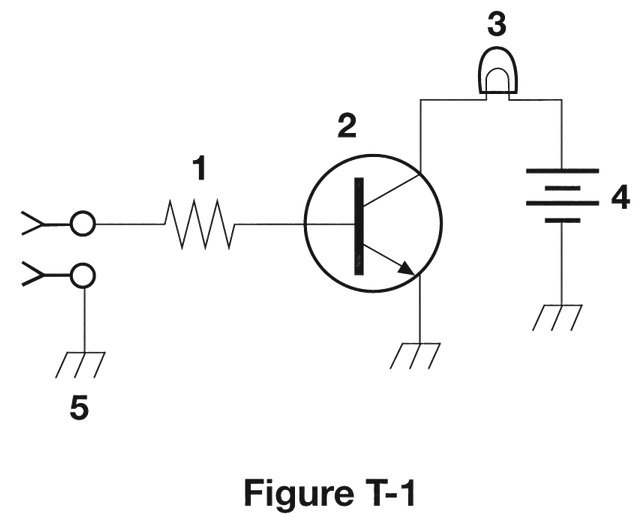
\includegraphics[width=0.5\textwidth]{tech/images/t1.png} 



    What is component 2 in figure T-1?
\begin{enumerate}[label=\Alph*)]
    \item Resistor
    \item \textbf{Transistor}
    \item Indicator lamp
    \item Connector
\end{enumerate}
\end{tcolorbox}

\subsubsection{Intuitive Explanation}
Imagine you’re looking at a LEGO set, and you’re trying to figure out what each piece does. Component 2 in figure T-1 is like the brain of the circuit—it’s the transistor! Just like how your brain controls your body, the transistor controls the flow of electricity in the circuit. It’s not just a simple resistor (which is like a speed bump) or a lamp (which just lights up). It’s the superstar that makes decisions!

\subsubsection{Advanced Explanation}
In electronic circuits, a transistor is a semiconductor device used to amplify or switch electronic signals and electrical power. It is composed of semiconductor material usually with at least three terminals for connection to an external circuit. In figure T-1, component 2 is identified as a transistor based on its symbol and placement within the circuit. 

The transistor operates by using a small input current or voltage to control a larger current flow, making it a crucial component in amplification and switching applications. The symbol for a transistor typically includes three terminals: the emitter, base, and collector. The specific type of transistor (e.g., NPN or PNP) can be determined by the direction of the arrow in the symbol.

% Diagram prompt: Generate a diagram showing the symbol of a transistor with labeled terminals (emitter, base, collector) and its placement in a simple circuit.